\section{Dropout}
Overfitting'i azaltmak için kullanılan bir düzenleme tekniğidir. Ağın öğrenme sürecinde rastgele seçilen nöronları devre dışı bırakarak ağın genelleme yeteneğini artırır. Bu, ağın farklı altkümelerini kullanarak birden fazla model öğrenmesini simüle eder. Bu süreç boyunca, her bir nöronun çıktısına "dropout" olasığı uygulanır. Bu olasılık nöronun eğitim sırasında geçerli iterasyonda kullanılmama olasılığını belirler. Genelde tam bağlı katmanlardan sonra kullanılarak bağlar koparılır. Böylece düğümler birbirleri hakkında daha az bilgiye sahip olur, birbirleri arasındaki ağırlık değişimlerinden daha az etkilenirler.

\begin{figure}[h]
    \centering
    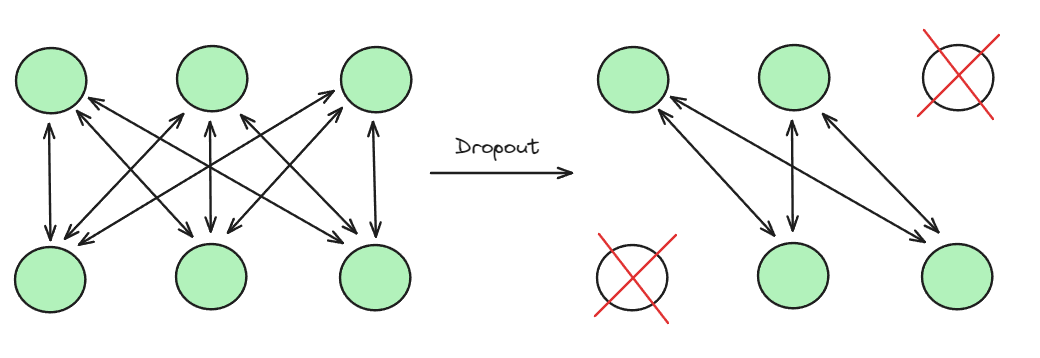
\includegraphics[width=1\textwidth]{images/dropout_layer.png}
    \caption{Dropout katmanı.}
    \label{fig:enter-label}
\end{figure}

\newpage